
\vspace{0.5cm}

\begin{figure}[]
  \centering
  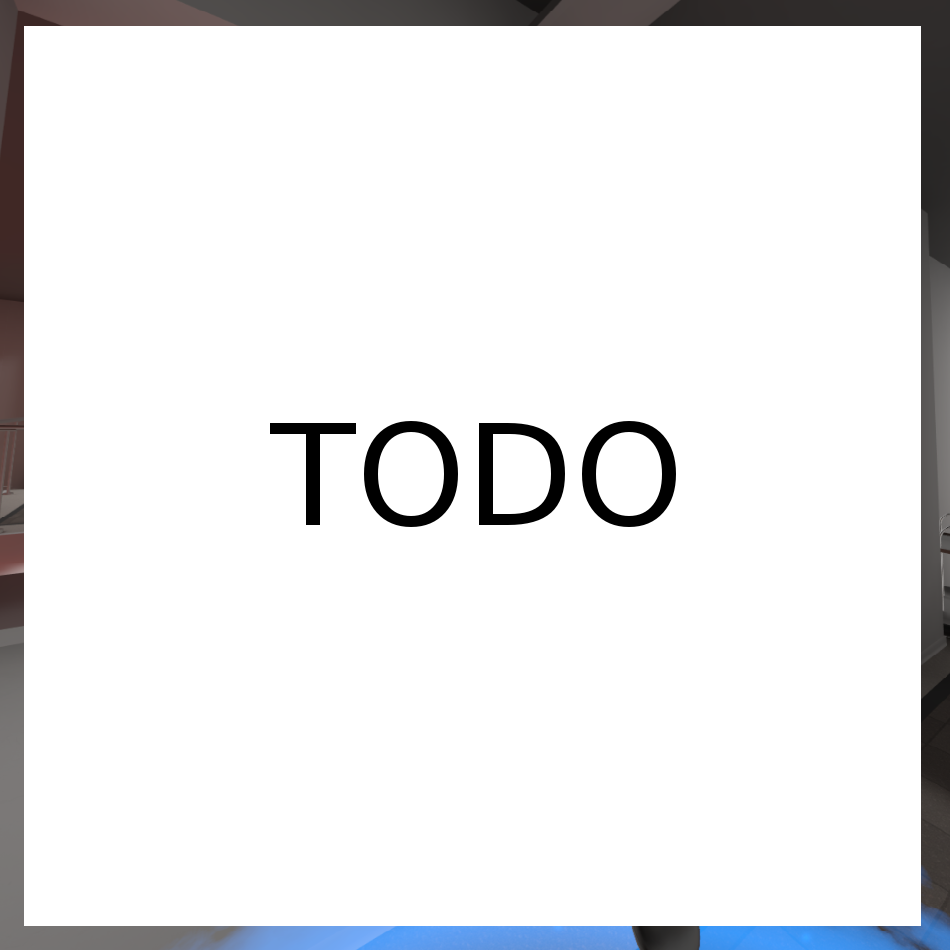
\includegraphics[width=0.5\textwidth]{images/todo.png}
  \caption{This is an example ToDo picture.}
  \label{fig:todo}
\end{figure}

Hypotheses and sub-hypotheses can be formulated like this:

\begin{hypothesis}
\label{hyp:test}
This is a hypothesis.
\end{hypothesis}

\begin{shypothesis}
\label{shyp:test}
This is a sub-hypothesis.
\end{shypothesis}

Hypothesis \cref{hyp:test} is very importance and must be referenced in the text.



Wie im zweiten Kapitel beschrieben, lassen sich durch die Größe der WIM mit Hilfe Fitt`s Law implizit Rückschlüsse auf das Kriterium der Bearbeitungszeit ziehen. Da der Teleport selbst nämlich keinerlei Zeit in Anspruch nimmt, bestimmt die Zeit zur Zielauswahl in der WIM die Dauer der Reise. Diese muss also möglichst gering gehalten werden. In diesem Falle wird wie bereits beschrieben ein maximaler Index of Difficulty von 5 vorausgesetzt, um eine zügige Interaktion zu gewährleisten. Diese wird Interaktion ist in Form von verschiedenen Auswahlstrahlen (genauer beschrieben im nächsten Unterpunkt) in der WIM jedoch eine einfache 3D-Zielbewegung mit fünf Freiheitsgraden für deren Effizienz umfangreiche wissenschaftliche Erkenntnisse vorliegen. Aus aktuelle Arbeiten zu 3D-Selektionsaufgaben (Teather und Stürzlinger (2011), Grossman und Balakrishnan (2004)) kann man für einen Schwierigkeitsindex von 4 eine Bearbeitungsdauer von ca. 2 Sekunden ableiten.




\def\rot{\rotatebox}

%https://tex.stackexchange.com/questions/98388/how-to-make-table-with-rotated-table-headers-in-latex
 \begin{table}[H]
 \centering
 \begin{tabular}{|c|l|r|r|r|r|}
 \hline
 & \multicolumn{1}{c|}{\rot{90.0}{Sichtbarkeit}} & \multicolumn{1}{c|}{Text} & \multicolumn{1}{c|}{Text} & \multicolumn{1}{c|}{Text} & \multicolumn{1}{c|}{text}\\
 \hline
 \parbox[t]{2mm}{\multirow{3}{*}{\rotatebox[origin=c]{90}{rota}}} & text &&&&\\
 & text &&&&\\
 & text &&&&\\
 \hline
 \end{tabular}
 \end{table}